\section{Boltzmann Machine}
In this thesis we are going to use a slightly different type of neural network, called a Boltzmann machine. First major contribution to Boltzmann machines comes from G. E Hinton and T.J. Sejnowski in 1983 \cite{ancoopcomp}. The neural net is a generative model which learns by matching the probability distribution of its inputs. 

\subsection{Structure and training}

A Boltzmann machine has interconnected nodes within a layer.

\begin{figure}[H]
    \centering
    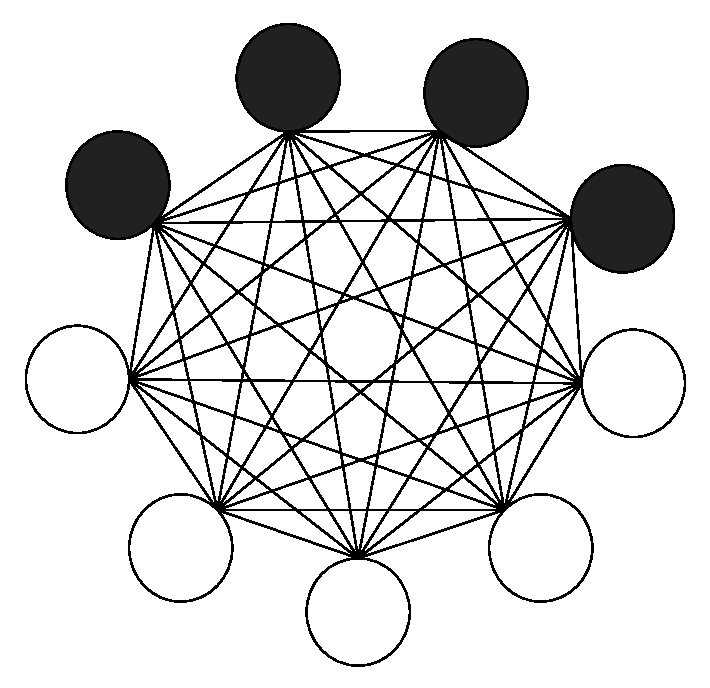
\includegraphics[width=0.7\textwidth]{Figures/Drawn/machinelearning/boltzmann1.pdf}
    \caption{A unrestricted Boltzmann machine where every node is connected. Here the black nodes are the visible layer while the white nodes constitute the hidden layer. }
    \label{fig:boltz1}
\end{figure}

The nodes are binary, being able to take the value $0$ or $1$, have a weights $w_{ij}$ for connection strength between node $v_i$ and $h_j$ and biases $a_i$ for the visible layer and $b_j$ for the hidden layer. For a system of $N_h$ hidden neurons and $N_v$ visible neurons we have the probability distribution of nodes taking the value $1$ defined as

\begin{equation}
    P(\boldsymbol{v},\boldsymbol{h}) = \frac{1}{Z} e^{-E(\boldsymbol{v},\boldsymbol{h})} \; ,
\end{equation}

where the energy of the model is given by

\begin{equation}
    E(\boldsymbol{v},\boldsymbol{h}) = -\sum_i^{N_v} a_i v_i - \sum_j^{N_h} b_j h_j -\sum_i^{N_v} \sum_j^{N_h} v_i w_{ij} h_j
\end{equation}

and the normalization factor

\begin{equation}
    Z = \sum_{ \boldsymbol{v}, \boldsymbol{h}} e^{-E(\boldsymbol{v},\boldsymbol{h})} \; ,
\end{equation}

where we sum over all possible states of the model, which increases exponentially as $2^{(N_v + N_h)}$. The marginal distribution over the visual layer can be written as

\begin{equation}
    P(\boldsymbol{v}) = \sum_{\boldsymbol{h}} \frac{1}{Z} e^{-E(\boldsymbol{v}, \boldsymbol{h})}
\end{equation}

To train a Boltzmann machine we need to have a cost function that compares the predicted distribution of the model and the actual distribution of the data set. As such we will use the Kullback-Leibler divergence as a cost function:

\begin{equation}
    KL(\boldsymbol{W}, \boldsymbol{a}, \boldsymbol{b}) = \sum_{(\boldsymbol{v}, \boldsymbol{h})} R(\boldsymbol{v}) \log{\frac{R(\boldsymbol{v})}{P(\boldsymbol{v})}} \; ,
\end{equation}

where $R(\boldsymbol{v})$ is the distribution we want to approximate and $P(\boldsymbol{v})$ is the distribution of the neural network model. Following the derivations of A.L. Yuille \cite{boltzderv} we have that

\begin{equation}\label{eq:costderv}
    \frac{ \partial KL(\boldsymbol{W}, \boldsymbol{a}, \boldsymbol{b})}{\partial w_{ij}} = - \sum_{(\boldsymbol{v}, \boldsymbol{h})} \frac{ R(\boldsymbol{v})}{P( \boldsymbol{v})} \frac{\partial P( \boldsymbol{v})}{\partial w_{ij}} \; ,
\end{equation}

where we further have

\begin{equation}
    \frac{\partial P(\boldsymbol{v})}{\partial w_{ij}} = \frac{1}{Z} \frac{\partial}{\partial w_{ij}} \sum_{\boldsymbol{h}} e^{-E(\boldsymbol{v}, \boldsymbol{h})} - \frac{1}{Z}  \sum_{\boldsymbol{h}} e^{-E(\boldsymbol{v}, \boldsymbol{h})} \frac{\partial \log{Z} }{\partial w_{ij}}
\end{equation}

which we can express as

\begin{equation}
    \frac{\partial P(\boldsymbol{v})}{\partial w_{ij}} = - \sum_{\boldsymbol{h}} v_i h_j P(\boldsymbol{v},\boldsymbol{h}) + \sum_{\boldsymbol{h}} \left [ P(\boldsymbol{v},\boldsymbol{h}) \sum_{\boldsymbol{v},\boldsymbol{h}} v_i h_j P(\boldsymbol{v},\boldsymbol{h})  \right ] \; .
\end{equation}

Then
\begin{equation} \label{eq:modelderv}
     \frac{\partial P(\boldsymbol{v})}{\partial w_{ij}} = - \sum_{\boldsymbol{h}} v_i h_j P(\boldsymbol{v},\boldsymbol{h}) + P(\boldsymbol{v},\boldsymbol{h}) \sum_{\boldsymbol{v},\boldsymbol{h}} v_i h_j P(\boldsymbol{v},\boldsymbol{h}) \; .
\end{equation}

Using the result of equation \ref{eq:modelderv} in equation \ref{eq:costderv} we get that

\begin{equation}
    \frac{ \partial KL(\boldsymbol{W}, \boldsymbol{a}, \boldsymbol{b})}{\partial w_{ij}} = \sum_{\boldsymbol{v},\boldsymbol{h}} v_i h_j \frac{P(\boldsymbol{v},\boldsymbol{h})}{P(\boldsymbol{v})} R(\boldsymbol{v}) - \left [\sum_{\boldsymbol{v},\boldsymbol{h}} R(\boldsymbol{v})\right ] \sum_{\boldsymbol{v},\boldsymbol{h}} v_i h_j P(\boldsymbol{v},\boldsymbol{h}) \; ,
\end{equation}

which we can simplify

\begin{equation}
    \frac{ \partial KL(\boldsymbol{W}, \boldsymbol{a}, \boldsymbol{b})}{\partial w_{ij}} = \sum_{\boldsymbol{v},\boldsymbol{h}} v_i h_j P(\boldsymbol{h} | \boldsymbol{v}) R(\boldsymbol{v}) - \sum_{\boldsymbol{v},\boldsymbol{h}} v_i h_j P(\boldsymbol{v},\boldsymbol{h}) \; ,
\end{equation}

where we require that

\begin{equation}
     \frac{\partial \log{Z} }{\partial w_{ij}} = \sum_{\boldsymbol{v},\boldsymbol{h}} v_i h_j P(\boldsymbol{v},\boldsymbol{h}) \; .
\end{equation}
We then define the expectation, or correlation, values

\begin{equation}
    \left < v_i h_j \right >_{\text{data}} = P(\boldsymbol{h} | \boldsymbol{v}) R(\boldsymbol{v})
\end{equation}

and

\begin{equation}
    \left < v_i h_j \right >_{\text{model}} = P(\boldsymbol{v}, \boldsymbol{h}) \; .
\end{equation}

This gives us the update rule

\begin{equation}\label{eq:wdiff}
    \Delta w_{ij} = - \eta \left ( \left < v_i h_j \right >_{\text{data}} - \left < v_i h_j \right >_{\text{model}} \right ) \; . 
\end{equation}
\subsection{Restricted Boltzmann machine}
Estimating $ \left < v_i h_j \right >_{\text{data}}$ and $ \left < v_i h_j \right >_{model}$ is done by Gibbs sampling, which is explained in a later chapter, but can be inefficient and take a long time to converge for complex models. Removing the weights between nodes within the same layer we can alleviate much of the computational cost of training. This type of Boltzmann machine is called a restricted Boltzmann machine, or RBM:

\begin{figure}[H]
    \centering
    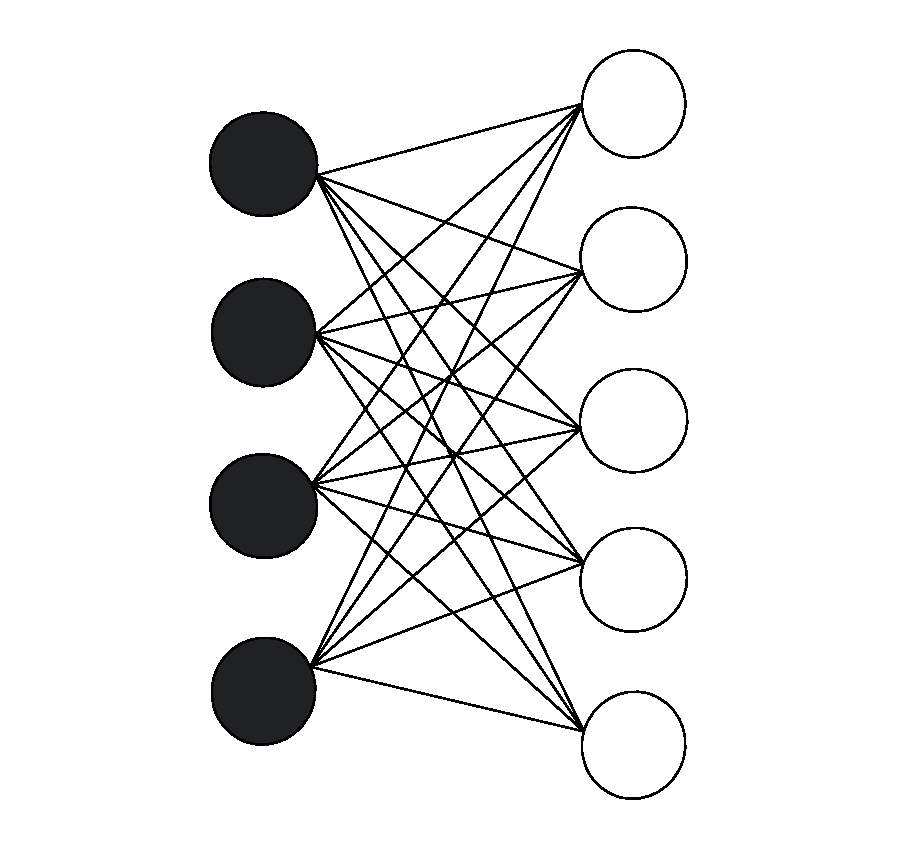
\includegraphics[width=0.7\textwidth]{Figures/Drawn/machinelearning/boltzrest.pdf}
    \caption{A restricted Boltzmann machine where there are no connections between nodes within the same layer. The white nodes are hidden while the black ones are the visible nodes.}
    \label{fig:boltzrest}
\end{figure}

Making the nodes independent of nodes in the same layer means we can write the conditional distributions as

\begin{equation}
    P(\boldsymbol{v} | \boldsymbol{h} ) = \prod_{i \in \boldsymbol{v}} P(v_i | \boldsymbol{h} ) \; , 
\end{equation}

and
\begin{equation}
    P(\boldsymbol{h} | \boldsymbol{v} ) = \prod_{j \in \boldsymbol{h}} P(h_j | \boldsymbol{v} ) \; .
\end{equation}

In a RBM we first have a forward pass where we insert the input data into the visual layer, then we sample the hidden layer by the distribution:

\begin{equation}
    p(h_j^{(0)} = 1 | \boldsymbol{z}_{v}^{(0)}) = \sigma\left (\boldsymbol{z}_{v}^{(0)} \otimes \boldsymbol{W} + \boldsymbol{b} \right ) \; , 
\end{equation}

where our activation function $\sigma$ is the Sigmoid function \ref{Tab:sigmoid}. The index $(0)$ indicate that it is the first pass-through the neural network. As the nodes are binary we then take a sample from $p(h_j^{(0)}=1 | \boldsymbol{z}_v^{(0)} )$ as a Bernoulli distribution, which means each $z_{h, j}^{(0)}$ takes the value $1$ with probability $h_j^{(0)}$. After the forward pass we have a backward pass where we sample from the hidden layer

\begin{equation}
    p(v_j^{(1)} = 1 | \boldsymbol{z}_{h}^{(0)}) = \sigma\left (\boldsymbol{z}_{h}^{(0)} \otimes \boldsymbol{W} + \boldsymbol{a} \right ) \; , 
\end{equation}

where we then convert it to binary values as well. For a continuous valued output it is optional to let the last visual output to remain as a probability distribution. Estimating $\left < v_i h_j \right >_{\text{data}}$ is done by sampling from $P(\boldsymbol{h} | \boldsymbol{v} )$

\begin{equation}
    \left < \boldsymbol{v} \boldsymbol{h} \right >_{\text{data}} = \boldsymbol{z}_v^{(0)} \otimes p(\boldsymbol{h}^{(0)} | \boldsymbol{z}_{v}^{(0)})
\end{equation} \; ,

while estimating $ \left < v_i h_j \right >_{\text{model}}$ requires that we let the model sufficiently affect the output. To do this we do Gibbs sampling through $k$ iterations of the forward and backward passes. Then we have

\begin{equation}
    \left < \boldsymbol{v} \boldsymbol{h} \right >_{\text{model}} = \boldsymbol{z}_v^{(k)} \otimes p(\boldsymbol{h}^{(k)} | \boldsymbol{z}_{v}^{(k)})
\end{equation} \; .

And from \ref{eq:wdiff} the change in weight becomes

\begin{equation}\label{eq:rbm_change_weight}
  \Delta \boldsymbol{W} = \eta \left [\boldsymbol{z}_v^{(0)} \otimes p(\boldsymbol{h}^{(0)} | \boldsymbol{z}_{v}^{(0)}) - \boldsymbol{z}_v^{(k)} \otimes p(\boldsymbol{h}^{(k)} | \boldsymbol{z}_{v}^{(k)}) \right ] \; .
\end{equation}
\subsection{Neural net quantum state}

To apply the restricted Boltzmann machine on a quantum mechanical system, a way to represent the system's state is needed. As the visual layer the output of the machine, and can here be viewed as the collapsed state of the system after measurement, we use the marginal distribution of the visual layer, the probability distribution of the visual layer states given the state of the hidden layer, to represent the wavefunction of the system.

\begin{align}
  \Psi_{rbm}(\boldsymbol{v}) &=\frac{1}{Z} \sum_{\boldsymbol{h}} \exp{-E(\boldsymbol{v}, \boldsymbol{h})} \\
                             &=\frac{1}{Z} e^{-\sum_i^{N_v} \frac{(x_i - a_i)^2}{2}} \prod_j^{ N_h } (1 + e^{b_j + \sum_i^{N_v} x_i w_{ij}})\; ,
  \label{eq:nqs_rbm}
\end{align}

This is most often referred to as a neural net quantum state, or abbreviated NQS.

\subsection{Minimizing local energy}

We want a restricted boltzmann machine to match the distribution of the ground state of a quantum mechanical systems. This poses a problem with the use of the change in weight, \ref{eq:rbm_change_weight}, as we do not have any data to train the model on. Instead we will use the variational principle with the fact that

\begin{equation}
  E \left [ \Psi_{rbm} \right ] \geq E_0 \; ,
  \label{eq:train_rbm_vp}
\end{equation}

where $\Psi_{rbm}$ is the machine state and $E_0$ is the ground state of the quantum system we want the machine state to match. Because of \ref{eq:train_rbm_vp} we can variationly minimize the expected energy and be certain that it approaches the ground state. This poses another problem, though, because the machine state is not directly accessible, but one can take samples from the machine's distribution. So instead of using the machine state directly, one approximates it by a sufficient amount of samples, essentially taking repeated measurements of the system and constructing the wavefunction from the result. For $N$ total number of samples, and $M_k$ the number of samples that are the basis state $\ket{b_k} \in \boldsymbol{B}$, then we have the approximate machine state:

\begin{equation}
  \Psi_{rbm} \approx \sqrt{\frac{M_0}{N}} \ket{b_0} + \sqrt{\frac{M_1}{N}}\ket{b_1} + \dots + \sqrt{\frac{M_N}{N}}\ket{b_N} \; ,
  \label{eq:approximate_machine_state}
\end{equation}

where we assume the wavefunction is real and positive definite. We use the samples to then approximate the energy by finding the expectation value of their local energy. The local energy is defined as:

\begin{equation}
  E_L(s) = \frac{\bra{s}H\ket{\Psi_{rbm}}}{\braket{s}{\Psi_{rbm}}} \; ,
  \label{eq:rbm_local_energy}
\end{equation}

where $\bra{s}$ is a sample. The system energy can then be approximated

\begin{equation}
  \langle E \rangle \approx \langle E_L \rangle = \frac{1}{N} \sum_{k=0}^{N} E_L(s_k) \; .
  \label{eq:rbm_energy}
\end{equation}

So minimizing the energy of the machine state can be done through minimizing the local energy. To derive the cost function, our gradient for the gradient decent calculations, we will take inspiration from this derivation \cite{DerivationGradient} of unknown author. Starting of with the expected value of the hamiltonian

\begin{equation}
  \langle H \rangle = \frac{\int \mathrm{d}\Psi(X)^* H \Psi(X)}{\int\mathrm{d}X \Psi^*(X)\Psi(X)} \; ,
  \label{eq:expected_hamiltonian}
\end{equation}

we then have the derivative by using the chain rule

\begin{equation}
  \frac{\partial}{\partial{\alpha}}\langle H \rangle = \frac{\int\mathrm{d}X \Psi^*_{\alpha}H\Psi + \Psi^*H\Psi_{\alpha}}{\int\mathrm{d}X\Psi^*\Psi} - \frac{\left ( \int\mathrm{d}X\Psi^*H\Psi\right )\left ( \int\mathrm{d}X\Psi_{\alpha}\Psi + \Psi^*\Psi_{\alpha}\right )}{\left ( \int\mathrm{d}X\Psi^*\Psi\right )^2} \; ,
  \label{eq:expected_derivative}
\end{equation}

 where $\Psi_{\alpha}$ is used to denote $\frac{\partial\Psi}{\partial\alpha}$. Now we expand the integrals of the numerator of the second term by $\Psi^*\Psi$ and we get

\begin{equation}
  \frac{\partial}{\partial\alpha} \langle H\rangle = 
\frac{\int \mathrm{d}X\, \Psi_\alpha^* H \Psi + \Psi^* H\Psi_\alpha}{\int \mathrm{d}X\, \Psi^* \Psi }
- \left\langle E_L\right\rangle \left\langle \frac{\partial}{\partial\alpha} \ln |\Psi|^2\right\rangle \; .
  \label{eq:first_expand}
\end{equation}

We then use the fact that the hamiltonian is Hermitian:

\begin{equation}
  \int \mathrm{d}X\, \Psi^* H\Psi_\alpha=\int \mathrm{d}X\, \Psi_\alpha (H\Psi)^* \; ,
  \label{eq:Hermitian_hamiltonian}
\end{equation}

and we get

\begin{equation}
  \frac{\partial}{\partial\alpha} \langle H\rangle = 
\frac{\int \mathrm{d}X\, \Psi_\alpha^* H \Psi + \Psi_\alpha (H\Psi)^*}{\int \mathrm{d}X\, \Psi^* \Psi }
- \left\langle E_L\right\rangle \left\langle \frac{\partial}{\partial\alpha} \ln |\Psi|^2\right\rangle .
  \label{eq:first_expand_hermit}
\end{equation}

then expanding the first terms numerator integrals by $\Psi^*\Psi$ we end up with

\begin{align}
\frac{\partial}{\partial\alpha} \langle H\rangle &= 
\left\langle \frac{\Psi_\alpha^*}{\Psi^*} \frac{H \Psi}{\Psi}+ \frac{\Psi_\alpha}{\Psi} \left(\frac{H\Psi}{\Psi}\right)^*\right\rangle
- \left\langle E_L\right\rangle \left\langle \frac{\partial}{\partial\alpha} \ln |\Psi|^2\right\rangle
\\
 &= 
\left\langle \frac{\Psi_\alpha^*}{\Psi^*} E_L+ \frac{\Psi_\alpha}{\Psi} E_L^*\right\rangle
- \left\langle E_L\right\rangle \left\langle \frac{\partial}{\partial\alpha} \ln |\Psi|^2\right\rangle \; .
\end{align}

If we now assume that $\Psi$ is real, and then $E_L$ would also be real, we can shorten the gradient

\begin{equation}
  \frac{\partial}{\partial\alpha} \langle H \rangle = 2\left(\langle E_L \frac{1}{\Psi}\frac{\partial\Psi}{\partial\alpha}\rangle - \langle E_L \rangle\langle\frac{1}{\Psi}\frac{\partial\Psi}{\partial\alpha}\rangle\right ) \; ,
  \label{eq:cost_function}
\end{equation}

where $\alpha$ then is our collection of weights and biases
\subsection{Change in weights and biases}

For practical use of the cost function \ref{eq:cost_function} defined above, we need to derive the change in weights and biases. With the fact that $\frac{1}{\Psi}\frac{\partial\ln{\Psi}}{\partial\alpha} = \frac{\partial\ln{\Psi}}{\partial\alpha}$ together with

\begin{equation}
  \ln{\Psi(\boldsymbol{v})} = -\ln{Z}-\sum_{i}^{N_v}\frac{(v_i-a_i)}{2}+\sum_{k}^{N_h} \ln{\left (1+\exp{b_k+\sum_j^{N_v}v_jw_{jk}}\right)} \; ,
  \label{eq:log_psi}
\end{equation}

we can then find that

\begin{gather}
  \frac{\partial}{\partial a_i} \ln{\Psi}= v_i - a_i\\
  \frac{\partial}{\partial b_j} \ln{\Psi}= \left (\exp{-b_j-\sum_k^{N_v}v_kw_{kj}}+1\right)^{-1} \\
  \frac{\partial}{\partial w_{ij}}\ln{\Psi} =v_i\left (\exp{-b_j-\sum_k^{N_v}v_kw_{kj}}+1\right)^{-1} \; . 
\end{gather}
